\documentclass[aspectratio=169]{beamer}

\usetheme{metropolis}
\setbeamertemplate{footline}{}
\setbeamertemplate{headline}{}

\title{Apache OpenWhisk}
\subtitle{Distributed Software Systems, 2024/25}
\author{Davide De Rosa}
\date{}

\begin{document}

\begin{frame}[plain]
    \titlepage
\end{frame}

%SLIDE 1: INTRODUCTION TO SERVERLESS COMPUTING
\section{Introduction to \\Serverless Computing}
\begin{frame}{Introduction to Serverless Computing}
\textbf{Serverless Computing} has transformed how we develop and deploy cloud applications. Traditional cloud computing required developers to manage virtual machines or containers, while \textbf{Serverless} eliminates this burden.\\
This model operates through \textbf{small}, \textbf{stateless functions} triggered by \textbf{events}, with the \textbf{cloud provider} managing backend infrastructure. Key benefits include:
\begin{itemize}
    \item \textbf{Autoscaling} to handle varying loads.
    \item A \textbf{pay-as-you-go} model, where costs align with actual function usage.
\end{itemize}
However, Serverless isn’t without its challenges. Cold starts, limited runtime languages, and debugging complexities still hinder its adoption.\\
Despite this, serverless computing has become integral to modern architectures, thanks to its simplicity and cost efficiency.
\end{frame}

%SLIDE 2: INTRODUCTION TO SERVERLESS COMPUTING
\begin{frame}{Introduction to Serverless Computing}
Over the past decade, cloud platform hosting has evolved significantly:
\begin{itemize}
    \item Initially, organizations purchased or rented physical servers to run applications, incurring costs for both the hardware and its maintenance.
    \item This shifted with the adoption of \textbf{virtualization}, which allowed a single physical server to function as multiple software-defined Virtual Machines (VMs), enhancing flexibility and resource utilization. \textbf{Containerization} emerged as a further refinement, combining aspects of virtualization with configuration management.
    \item The introduction of \textbf{Platform-as-a-Service} (\textbf{PaaS}) took abstraction further, freeing users from managing servers and deployment processes.
    \item The latest advancement, serverless computing, builds on \textit{PaaS} by enabling deployment of small code fragments that can autonomously scale, supporting the creation of self- scaling applications.
\end{itemize}
\end{frame}

%SLIDE 3: SERVERLESS ARCHITECTURE
\section{Serverless Architecture}
\begin{frame}{Serverless Architecture}
At its core, Serverless Computing revolves around simplicity and efficiency. Functions run in isolated containers, with each triggered by specific events like HTTP requests or database updates.
The process begins when an event triggers the platform:
\begin{itemize}
    \item An \textbf{event queue} receives the trigger and informs a dispatcher.
    \item The \textbf{dispatcher} assigns the function to a \textbf{worker node}.
    \item If a \textbf{worker} is free, it executes the function. Otherwise, the request is queued.
\end{itemize}
A load balancer ensures smooth operations, though challenges like resource contention and cold starts remain. To address this, providers pre-warm containers, minimizing latency during new invocations.    
\end{frame}

%SLIDE 4: SERVERLESS ARCHITECTURE
\begin{frame}{Serverless Architecture}
\centering
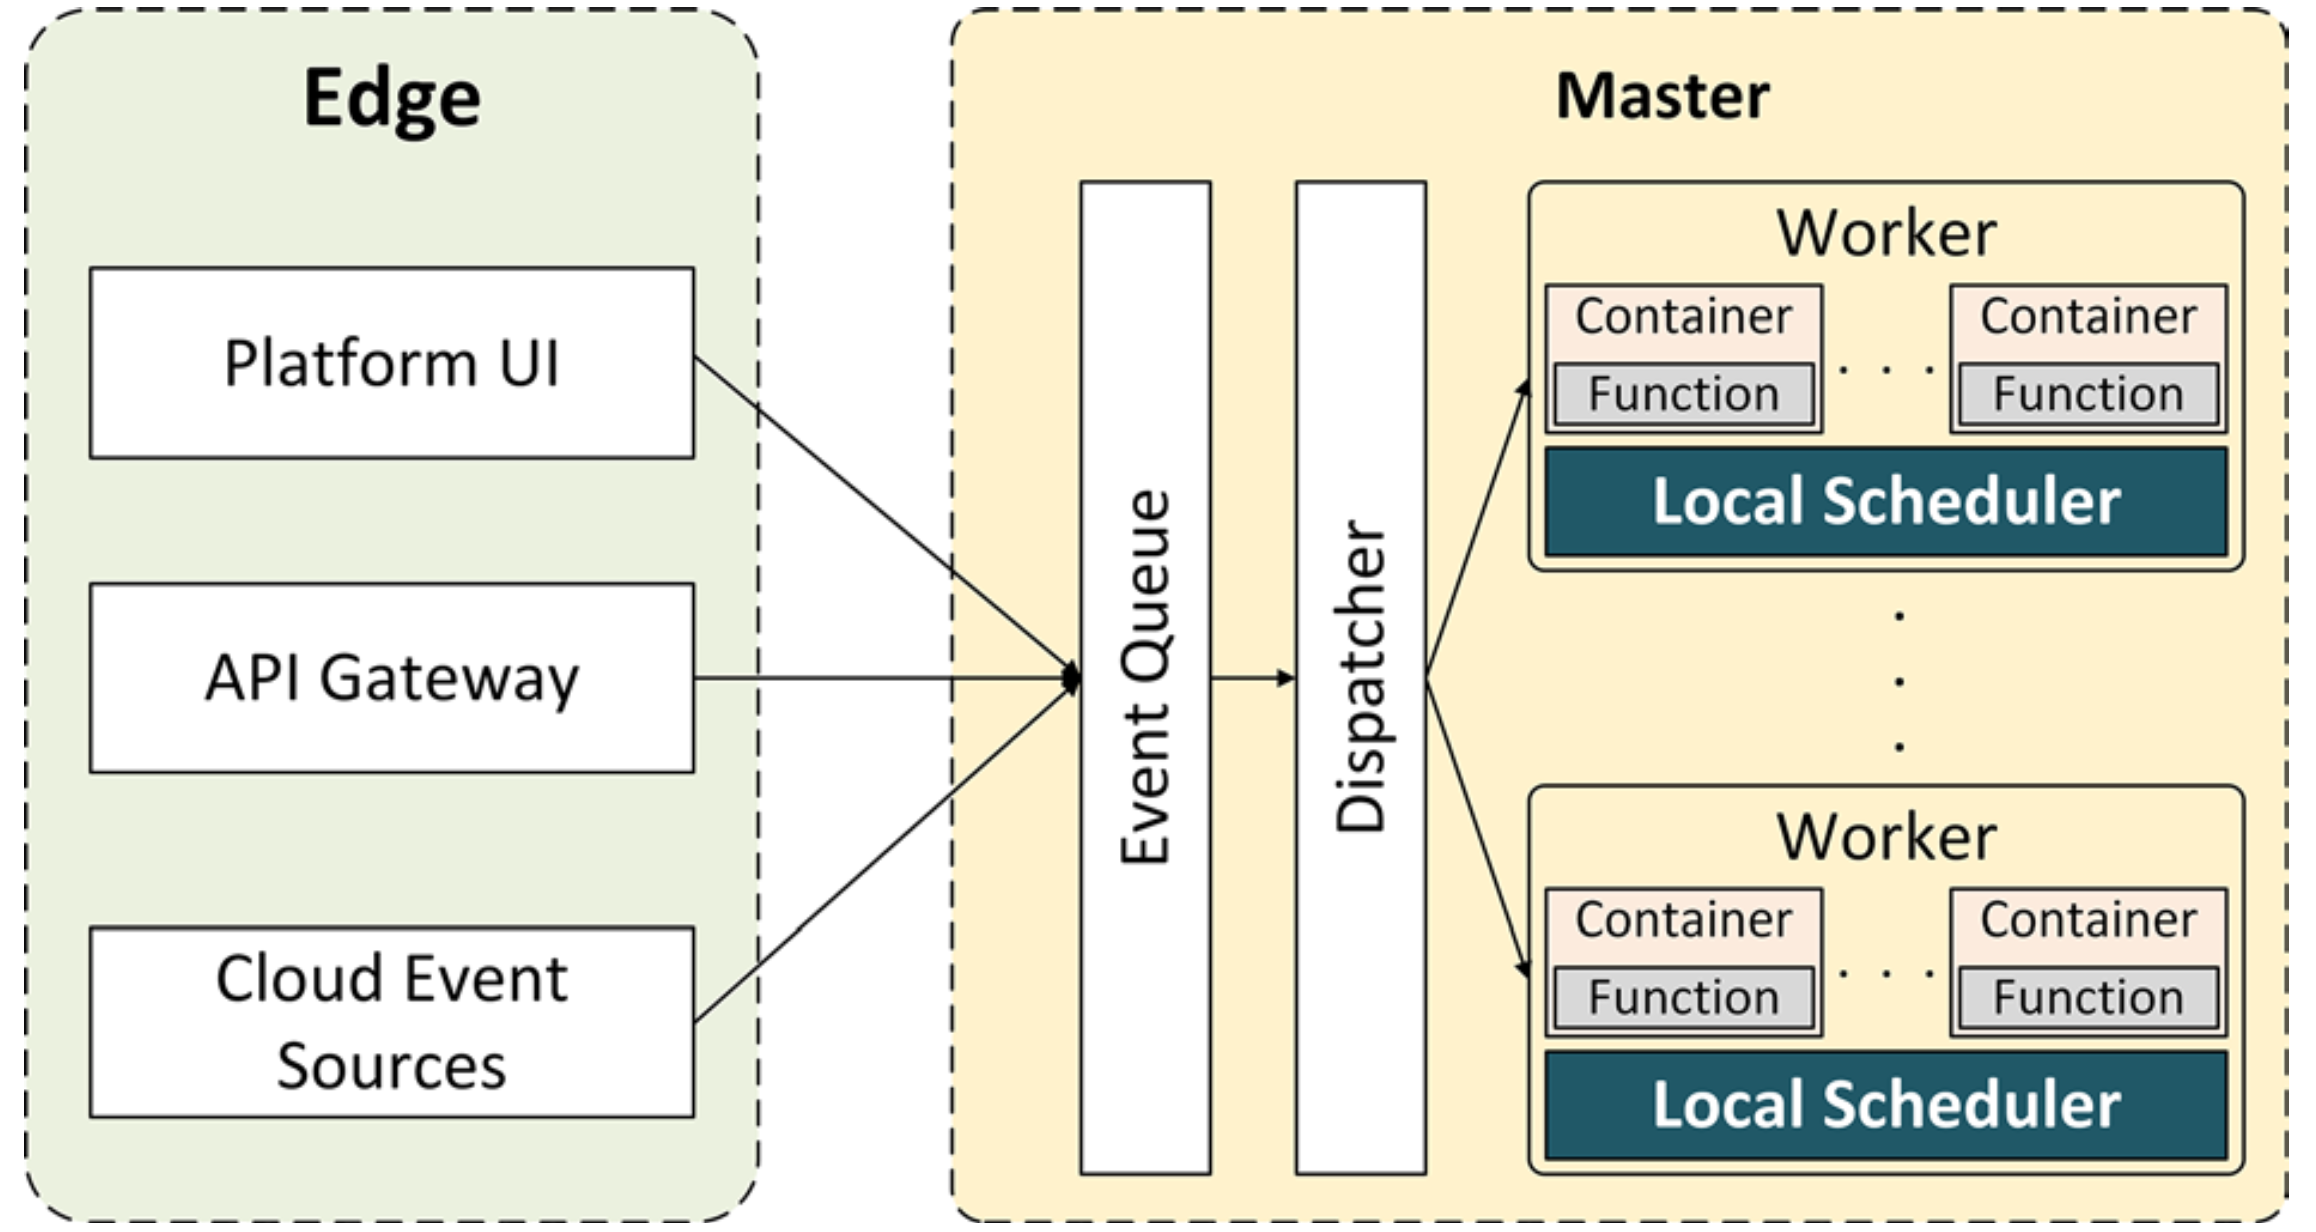
\includegraphics[width=0.8\textwidth]{img/arch.png}
\end{frame}

%SLIDE 5: APACHE OPENWHISK
\section{Apache Openwhisk}
\begin{frame}{Apache Openwhisk}
\textbf{Apache Openwhisk} is \textbf{IBM}’s \textbf{open-source} serverless platform. It competes with giants like \textit{AWS Lambda} and \textit{Google Cloud Functions} by offering flexibility and openness. Developers use Openwhisk to build applications requiring \textit{real-time processing}, \textit{IoT data handling}, or \textit{serverless APIs}.\\
Its design is \textbf{event-driven}, and its programming model is built around three elements:
\begin{itemize}
    \item \textbf{Actions}: Stateless functions that process events.
    \item \textbf{Triggers}: Events that activate functions.
    \item \textbf{Rules}: Bindings connecting triggers to actions.
\end{itemize}
What sets Openwhisk apart is its adaptability. It supports deployment on platforms like \textit{Kubernetes} and \textit{OpenShift}, and its CLI tool makes it accessible across operating systems.
\end{frame}

%SLIDE 6: APACHE OPENWHISK
\begin{frame}{Apache Openwhisk}
\centering
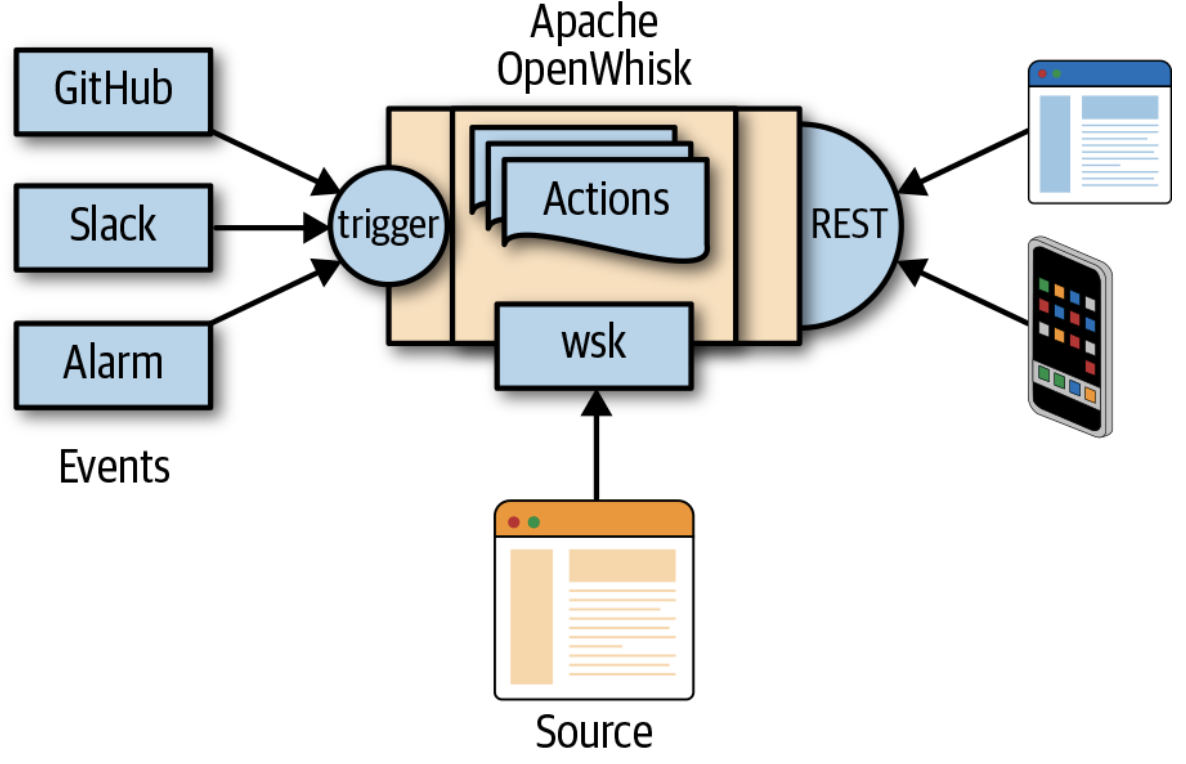
\includegraphics[width=0.75\textwidth]{img/ow_works.png}
\end{frame}

%SLIDE 7: APACHE OPENWHISK
\begin{frame}{Apache Openwhisk Key Features}
\begin{itemize}
    \item \textbf{Deploys Anywhere}: with its container-based architecture, Openwhisk offers versatile deployment options, supporting local setups and cloud infrastructures.
    \item \textbf{Supports Any Programming Language}: Openwhisk is compatible with a wide range of programming languages. For unsupported platforms or languages, users can easily create and customize executables using Docker.
    \item \textbf{Integration Support}: Openwhisk enables easy integration of developed Actions with popular services through pre-built packages.
    \item \textbf{Rich Function Composition}: functions written in multiple programming languages can be packaged with Docker for flexible invocation options, including synchronous, asynchronous, or scheduled execution.
    \item \textbf{Scalability and Resource Optimization}: Openwhisk allows Actions to scale instantly. Resources scale automatically to match demand, pausing when idle, so users only pay for actual usage with no costs for unused resources.
\end{itemize}
\end{frame}

\section{Apache Openwhisk \\Main Architectural Drivers}
\begin{frame}{Apache Openwhisk Main Architectural Drivers}
    ciao
\end{frame}

\section{Apache Openwhisk Architecture}
\begin{frame}{Apache Openwhisk Architecture}
    ciao
\end{frame}

\section{Competing solutions}
\begin{frame}{Competing solutions}
    ciao
\end{frame}

\section{Implementation}
\begin{frame}{Implementation}
    ciao
\end{frame}

\section*{References}
\begin{frame}{References}
    \begin{itemize}
        \item Etas: predictive scheduling of functions on worker nodes of apache openwhisk platform (Banaei, Ali and Sharifi, Mohsen), 2022
        \item Evaluating apache openwhisk-faas, Quevedo (Sebasti{\'a}n and Merch{\'a}n, Freddy and Rivadeneira, Rafael and Dominguez, Federico X), 2019
        \item Crypto currencies prices tracking microservices using apache OpenWhisk (Huy, Lam Phuoc and Saifullah, Saifullah and Sahillioglu, Marcel and Baun, Christian), 2021 
        \item Open-source serverless architectures: an evaluation of apache openwhisk (Djemame, Karim and Parker, Matthew and Datsev, Daniel), 2020
        \item LEARNING APACHE OPENWHISK: developing open serverless solutions (Sciabarr{\`a}, Michele), 2019
    \end{itemize}
\end{frame}
\end{document}